%% ****** Start of file aiptemplate.tex ****** %
%%
%%   This file is part of the files in the distribution of AIP substyles for REVTeX4.
%%   Version 4.1 of 9 October 2009.
%%
%
% This is a template for producing documents for use with 
% the REVTEX 4.1 document class and the AIP substyles.
% 
% Copy this file to another name and then work on that file.
% That way, you always have this original template file to use.

%\documentclass[aip,graphicx]{revtex4-1}
%\documentclass[aip,reprint]{revtex4-1}

%\usepackage{graphicx}

%\draft % marks overfull lines with a black rule on the right
%\documentclass[pre,aps,floatfix,authordate1-4,twocolumn]{revtex4-1}
%\documentclass[pre,aps,floatfix,authordate1-4]{revtex4-1}

\documentclass[aip,jcp,twocolumn]{revtex4}
%\documentclass[aip,jcp]{revtex4}
%\documentclass{article}



%\documentclass[aps,prl,preprint,groupedaddress]{revtex4}

\usepackage{rotating} 
\usepackage{times}
\usepackage{graphicx}
\usepackage{setspace}
\usepackage{amsmath}
\usepackage{epstopdf}
\usepackage[obeyFinal]{easy-todo}
\usepackage{csquotes}
\usepackage{mhchem}

%\usepackage{markdown} 

\begin{document}

% Use the \preprint command to place your local institutional report number 
% on the title page in preprint mode.
% Multiple \preprint commands are allowed.
%\preprint{}

\title{Accurate binding of calcium to phospholipid bilayers by effective inclusion of electronic polarization} %Title of paper

% repeat the \author .. \affiliation  etc. as needed
% \email, \thanks, \homepage, \altaffiliation all apply to the current author.
% Explanatory text should go in the []'s, 
% actual e-mail address or url should go in the {}'s for \email and \homepage.
% Please use the appropriate macro for the type of information

% \affiliation command applies to all authors since the last \affiliation command. 
% The \affiliation command should follow the other information.

\author{Josef Melcr}
\author{Hector Martinez-Seara Monne}
\author{Pavel Jungwirth}
\affiliation{Institute of Organic Chemistry and Biochemistry,
Academy of Sciences of the Czech Republic, 
Prague 6, Czech Republic}

\author{O. H. Samuli Ollila}
\email[]{samuli.ollila@helsinki.fi}
%\homepage[]{Your web page}
\affiliation{Institute of Organic Chemistry and Biochemistry,
Academy of Sciences of the Czech Republic, 
Prague 6, Czech Republic}
\affiliation{Institute of Biotechnology, University of Helsinki}


% Collaboration name, if desired (requires use of superscriptaddress option in \documentclass). 
% \noaffiliation is required (may also be used with the \author command).
%\collaboration{}
%\noaffiliation

\date{\today}

\begin{abstract}
  % insert abstract here
  \todo{Abstract directly from Joe's conference abstracts. To be rewritten.}
Classical molecular dynamics simulations give detailed information about membrane structure and dynamics. 
However, there is still a room for improvements in current force fields – it is known from the literature,
that the binding of ions, especially cations, to phopholipid membranes is overestimated in all classical models [1]. 
We suggest that the membrane-ion interactions can be corrected by including implicit electronic polarizability into the
lipid models through the electronic continuum correction (ECC) [2], which was already applied to monovalent and divalent
ions yielding models that feature correct ion pairing [3]. 
Using the electrometer concept [3, 4] and x-ray scattering form factors, our simulations point out that our hypothesis is
correct and ECC is indeed a missing important contribution in current classical lipid models. 
Moreover, the solid physical principles behind ECC are found not to hamper other relevant properties of a phospholipid bilayer. 
The new lipid model, "ECC-lipids", shows accurate binding affinity to sodium and calcium cations and headgroup order parameter response to bound charge. 
We also provide for the first time a realistic stochiometry of bound calcium cations to a POPC membrane, and their binding sites. 
This work will continue as an open collaboration project NMRlipids IV (http://nmrlipids.blogspot.fi).
\end{abstract}

%\pacs{}% insert suggested PACS numbers in braces on next line

\maketitle %\maketitle must follow title, authors, abstract and \pacs

% Body of paper goes here. Use proper sectioning commands. 
% References should be done using the \cite, \ref, and \label commands


% Here I write pseudo-article statements that will make the main argument.
% Beautiful polished sentences will be formed only afte we agree on these basic things
\section{Introduction}
Cation interactions with cellular membranes play a key role in several biological processes,
like in signal propagation in neurons and vesicle fusion.
Cation interactions with lipid bilayers serving as a model for cellular
membranes are thus widely studied with experimental \cite{cevc90,tocanne90,binder02,pabst07,uhrikova08}
and theoretical methods \cite{Berkowitz12,??}. General conclusion from experimental
studies has been that multivalent ions and lithium have weak specific binding in
phopholipid bilayers, while other monovalent ions do not essentially
bind \cite{cevc90,tocanne90,seelig90,binder02}. The presence of anoinic lipids, like PS or PG,
increase the concentration close to the bilayer and thus the amount of bound
ions, but do not affect the specific binding constant \cite{seelig90}.
The binding details, like binding sites and stoichiometry are not yet fully
resolved but interpretation of NMR and scattering experiments suggest that one
Ca2+ interacts mainly with the choline groups \cite{hauser76,hauser78,herbette84} of two
phospholipid molecules \cite{altenbach84}.

Classical molecular dynamics simulations have potential to solve the ion binding details
in lipid bilayers and reveal its relevance to various biological
problems \cite{bockmann03,bockmann04,??}. However, the available
molecular dynamics simulation models have a strong tendency to overestimate
cation binding on zwitterionic bilayers and none of them can reproduce the
experimental data with the accuracy required for the interpretation of
experiments \cite{catte16}. The overestimated specific cation binding also
makes zwitterionic bilayers effectively positively charged, which could
potentially lead to significant artefacts in applications.
Thus, there is a vast demand for classical molecular dynamics simulation
model which correctly reproduces cation binding in lipid bilayers. 

The lack of electronic polarizability from the classical MD simulation
models is a potential source of artefact, which could lead to overbinding
of cations. 
%Almost all lipid bilayer simulations reported in the literature 
%are done with force fields that represent interactions between atoms
%with pairwise additive empirical potential and exclude the electronic 
%polarizability \cite{SOME_review, FF_papers}.
The issue has been considered higly relevant since the early days of
lipid bilayer simulations and pioneering simulation studies scaled
the partial charges to effectively include electronic
polarizability \cite{jonsson86,egberts94}. The explicit inclusion of
electronic polarizability has been, however, turned to be 
practically complicated and implementations for lipids are rare \cite{chowdhary13}.

In this work we show that the cation overbinding in classical MD simulations
can be corrected by including electronic polarizability by using effective continuum
correction (ECC)~\cite{leontyev11} for polar region of zwitterionic lipid molecules.
This is essentially physicalle well justified version of partial charge scaling
implemented in early days of lipid and surfctant simulations \cite{jonsson86,egberts94}. 
The approach has been previously shown in to improve bulk performace of
ion models against neutron scattering data \cite{Jungwirth2015,kohagen14,kohagen16}.
The better bulk behaviour was not, however, sufficient to correct binding in lipid
bilayers \cite{catte16}. 
%motivation for its application to zwitterionic lipids like POPC.




\section{Methods}

\subsection{Electronic continuum correction for lipid bilayers}
According to the electronic continuum correction (ECC)\cite{leontyev11}, electronic
polarizability can be included in classical MD simulations by
placing all particles into a homogeneous dielectric continuum 
with a dielectric constant $\epsilon _{el}$. 
which is the electronic part of the dielectric constant of 
the media \cite{leontyev11}. Measurements of high frequency 
dielectric constant gives values of approximately $\epsilon _{el} \approx 2$ 
for almost any biomaterial \cite{some_original_work, leontyev11}. % that exists in living cells. 
Such a continuum can be easily included in standard MD simulation by
a formal transformation of partial charges 
\begin{equation}
  Q^{ECC} = f_q \cdot Q
\end{equation}
with a constant scaling factor $f_q = \epsilon _{el} ^{-1/2}$ 
effectively representing the newly introduced electronic continuum. 
The value measured for water, $\epsilon _{el} = 1.78$, gives 
a scaling factor of $f_q = 0.75$ \cite{some_orig_source, leontyev11}, which has been
successfully used to improve the performance of ion force fields \cite{kohagen14,kohagen16,??}. 

Here we apply the electronic continuum correction to lipid bilayers to accurately 
describe the lipid headgroup response to Na+ and Ca2+ concentrations \cite{catte16}. 
We use the Lipid14~\cite{dickson14} force field parameters as a starting point,
because they give the most realistic headgroup response with added cations 
and relatively realistic glycerol backbone and headgroup structures
when compared with other state of the art lipid models \cite{botan15,catte16}.
The partial atomic charges in Lipid14 were derived by fitting the electrostatic 
potential to its model quantum chemistry representation (RESP\cite{RESP_paper}) in vacuum.
If the charges are obtained by using RESP in an implicit solvent, 
they vary the most for the polar moieties \cite{maciejewski14}. 
In order to implicitly capture solvent induced polarization 
in models with fixed charges, 
we shall use the average of partial charges 
from both environments (i.e. vaccum and solvent),
so called implicitly polarized charges (IPolQ) \cite{ipolq2013}. 
By taking the charges of oxygen atoms in vacuum and implicit water solvent for POPC from \cite{maciejewski14}, 
we represent the IPolQ charges in the electronic continuum correction of the Lipid14 model
by increasing the scaling factor $f_q$ to $0.8$. 
\footnote{Depending on which QM method you arrive at values from 0.76 to 0.83, averages across atom types being around 0.78--0.80. Even though the methods are almost identical, authors of Lipid 14 find lower partial charges in vacuum than here -- so I prefer the higher value. As the choice of charges is arbitrary anyway, I use 0.80 as an approximate round value. The use of 0.78---.79 might be more appropriate, though.}

Hydrocarbon chains in Lipid14 and other lipids models are highly optimized and
give generally a good description for hydrophobic part of lipid bilayers
in various conditions \cite{ollila16},
in contrast to glycerol backbone and headgroup regions which require
some improvement in all available lipid models \cite{botan15}. 
To minimize the detuning of the highly optimized hydrocarbon
parameters, we apply ECC only
to the headgroup, glycerol backbone and carbonyl in acyl chains.
These regions are also the most polar parts in lipids and are expected
to most affect cation binding.   
%Because the biologically relevant cations like \ce{Na^+} and \ce{Ca^{2+}}
%are found to interact only with the phospholipid head group,
%and the accuracy of alkyl sidechains in Lipid14 model are satisfactory, 
%we exclude alkyl tails from our modifications. 

Mere scaling of partial charges in the modified region by the factor $f_q$ reduces the 
area per molecule to ??\todo{find the value}, which is significantly smaller than the
experimental value (\cite{}) and the original Lipid14 values (\cite{})\todo{Add the values}.  
The decrease of area was speculated 
\todo{SAMULI: Did you analyze the effect of this to hydration or did we only speculate?
JOE: I found a systematic decrease of water density in the heagroup region even if I kept APL constant.}
to arise from reduced hydration
of headgroup due to the lower polarity of molecules with scaled charges.
The hydration can be increased by decreasing the radius of atoms
by reducing the $\sigma$ parameters in Lennard-Jones potential for the selected atoms.
This allows water molecules to approach closer to lipid atoms and
have stonger electrostatic interactions with them.
\todo{SAMULI: This effect may have an official name. In that case we should mention it.}
Indeed, by reducing $\sigma$ with a scaling factor $f_\sigma = 0.89$ 
we increased the area per molecule
to a level close to experimental and original Lipid14 values. 
%\todo{Is there some justification for the below sentence?} 
%In line with the electronic continnum correction,
%the scaling factor for sigma parameters, $f_\sigma$,
%has to lay between $f_q$ and 1.


\subsection{Comparison to experimental data}
Structures sampled by individual lipid molecules in simulations were compared
to experimental data by using C-H bond order parameters \cite{ollila16}
\begin{equation}
S_{\rm CH}=\frac{3}{2}\langle \cos^2\theta -1 \rangle,
\end{equation}
where $\theta$ is the angle between C-H bond and membrane
normal and average is taken over all sampled configurations.

Bilayer dimensions were compared to experiments by using the
scattering form factor \cite{ollila16}
\begin{equation}
  F(q) = \int _{-D/2} ^{D/2} \left ( \sum _\alpha f_\alpha (q_z) n_\alpha (z) - \rho _s \right ) \exp (izq_z) \mathrm{d}z,
\end{equation}
where $f_\alpha(q_z)$ is the density of atomic scattering length, 
$\rho_s$ is the density of solvent scattering lenght,
$n_\alpha (z)$ is the number density of atom $\alpha$ and
$z$ is the distance from the membrane centre along its normal 
spanning the membrane with thickness $D$. 

Ion binding was compared between experiments and simulations by 
using lipid headgroup order parameters and ''electrometer concept'' 
introduced by Seelig et al. \cite{seelig87,catte16}.
The concept is based on the experimental observation that the 
order parameters of $\alpha$ and $\beta$ carbons in lipid headgroup
(see Fig. \ref{??} 
\todo{Figure with chemical structure and labeling to be added}) 
are proportional to the amount of bound charge
in lipid bilayer \cite{seelig87}. More recent analysis included also
the order parameter signs and concluded that the order parameters  
decrease with bound positive charge and increase with bound negative 
charge \cite{ollila16,catte16}. The observations are rationalized 
as a change of lipid headgroup dipole tilt to more vertical orientation
with bound positive charge and {\it vice versa} for negative charge \cite{seelig87}. 

%\todo{ongoing,Actual concentration of cations in simulation has yet to be estimated. 
%If it varies too much from the nominal concentration, I may need to tweak the scaling 
%factors, $f_q$ or only $f_\sigma$, to accomodate it. However, it is very unlikely, response 
%to the surfactant \ce{DHMDMAB} is OK. Big patches with loads of solvent are running at the 
%moment to guide me on the possible finite-size errors and this conc-error.
The used experimental data report order parameters as a function of
equilibrium cation concentration in the bulk solvent \cite{akutsu81,altenbach84}.
Such a condition is reached in simulations by adjusting
the simulation box size to dimensions large enough
that ion conceration reaches a clear plateau in the bulk solvent.
The concentrations in the units of $\mathrm{mol/l}$ were then 
determined as
\begin{equation}
  C_{eq}=\frac{C_{plateau}}{0.602},
\end{equation}
where plateau concentration is the number density in the units of $\mathrm{nm}^{-3}$.
\todo{SAMULI: Once we have to final results, we can probably say that
  the repeat distance is not far from the experimentally measured distance \cite{pabst07,uhrikova08}
  }

\subsection{Simulation details}

\todo{To be written}


\subsubsection{Simulations with cationic surfactants}
Automated topoly builder \cite{malde11} was first used to create pdb structure of
dihexadecyldimethylammonium bromide, C$_{12}$Cl$_{16}$$^+$N2C$_1$Br$^-$, molecule.
The AmberTools \cite{amber} was then used to generate the Amber force field
parameters from the pdb file. These were converted to Gromacs format by using
acpype tool \cite{acpype}. The partial charges were then manually modified
to approximately correspond the corresponding segments in Lipid14 \cite{dickson14}.
The surfactants were randomly mized with lipids to form bilayer structures with
mole fractions 10\%, 20\%, 30\%, 42\% and 50\% of surfctant in POPC bilayer.
Simulation parameters and force field for POPC was already used and
described previously \cite{catte16} and were downloaded from \cite{lipid14POPC0mMNaClfiles}.
The systems were simulated 100-200~ns at 313K and the first 20~ns of the trajectories
were excluded from the analysis as an equilibration period.
The simulations were ran with Gromacs 5~\cite{abraham15}. 
Simulation trajectories and parameters are available at \cite{??} \todo{To be uploaded to Zenodo}.

\section{Results and Discussion}

\subsection{Lipid bilayers without ions}
The scattering form factors, NMR order parameters and area per lipids calculated from 
the ECC corrected lipid model for POPC are compared to experiments and original
Lipid14 results in Fig. \ref{simVSexpNOions} and in Table~\ref{tab:apls}. 
%The optimal value for $f_\sigma$ was found by representing the overall membrane structure well
%by matching scattering form factors to experimental data~\cite{Petrache06, Kucerka08, Pabst10}.
The structural quality is comparable to the state of art lipid models available in literature \cite{ollila16},
thus we conclude that the ECC corrected lipid model reproduces the lipid bilayer structure
in liquid disordered phase with similar accuracy than other available models
\todo{Discussion to be finished when we have all the results in the figure}.
\begin{figure}[]
  \centering
  \includegraphics[height=8.5cm,angle=-90]{../Fig/form-f_exp-l14-eccl17.eps}
%  \caption{\label{fig:form-f}
%    X-ray scattering form factors from experiments~\cite{Kucerka2011} and simulations using Lipid14 and ECCLipids17 models.  }
%\end{figure}
%
%\begin{figure}[]
%  \centering
  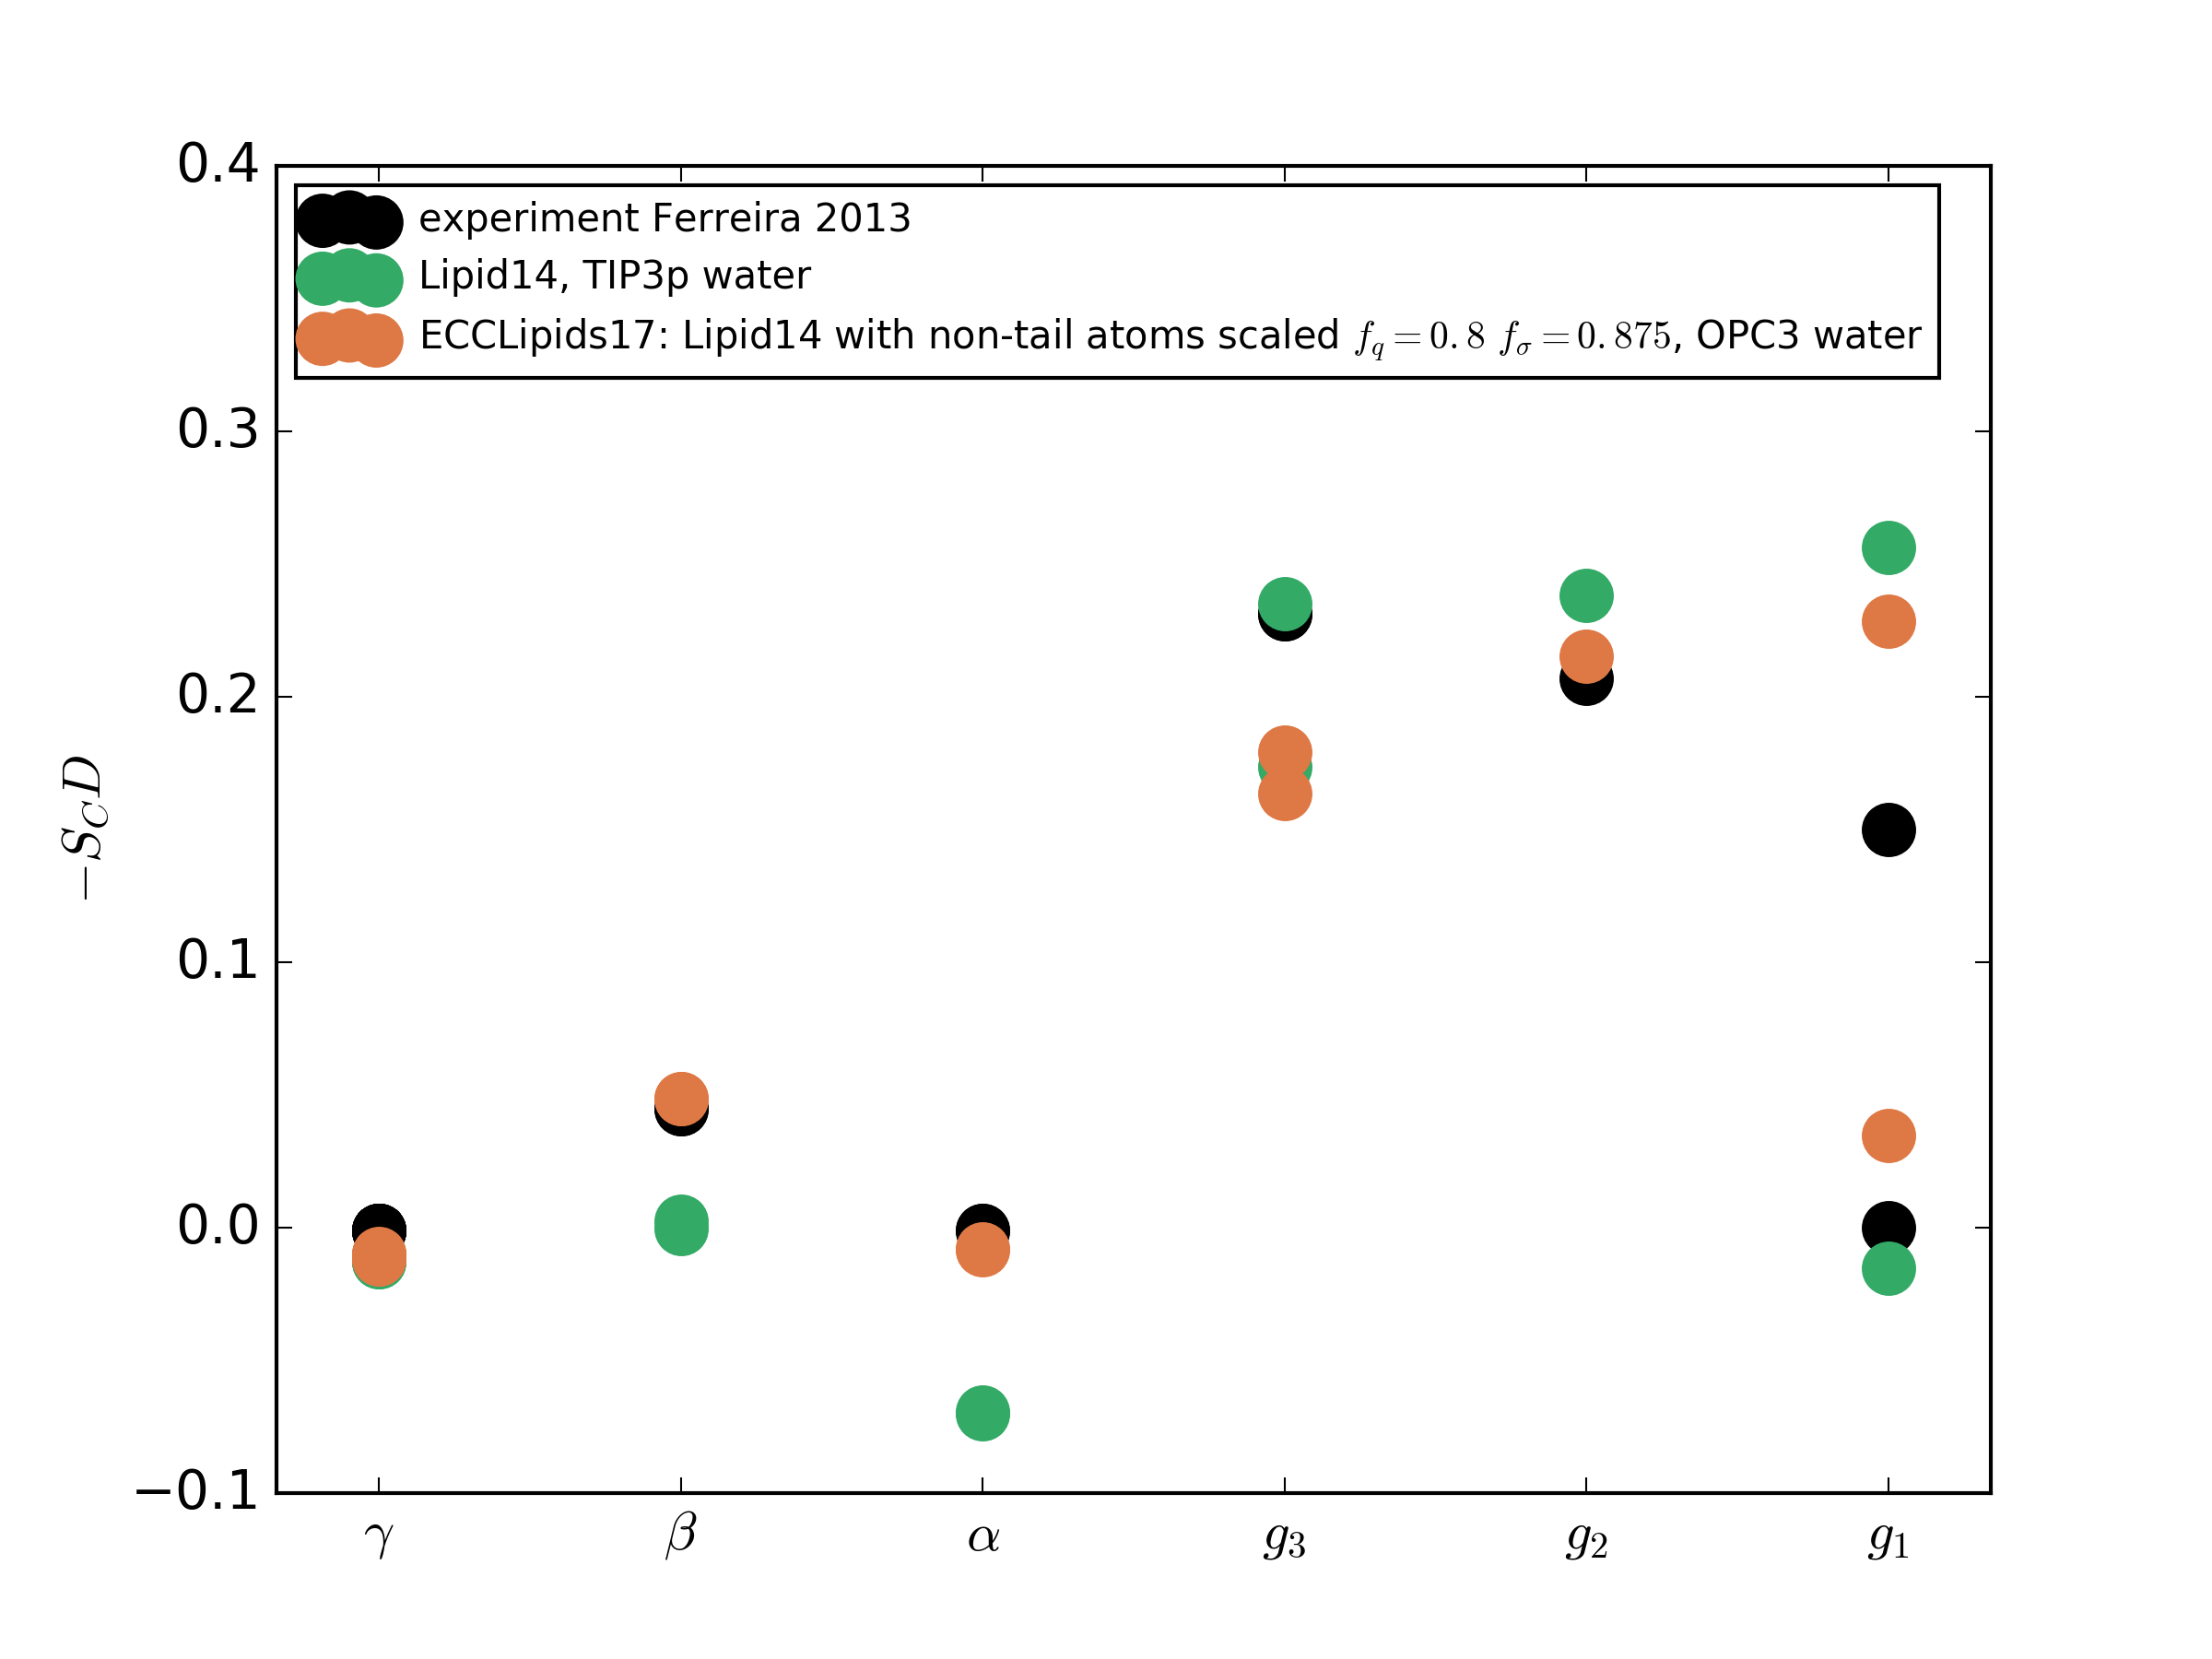
\includegraphics[width=9.0cm]{../Fig/ipython_nb/Headgr_OPs_exp-L14-ECCL17.png}
  \caption{\label{simVSexpNOions}
    X-ray scattering form factors from experiments~\cite{Kucerka2011} and simulations using Lipid14 and ECCLipids17 models. 
    Headgroup and glycerol backbone order parameters from simulations with Lipid14 \cite{dickson14} and EECLipid17 models
    compared with experimental order parameters from \cite{ferreira13}.}
  \todo{Add acyl chain order parameters, POPC chemical structure}
  \todo{Should we add the results from original lipid14?}
\end{figure}
%Area per molecules extracted from MD simulations and SPD model fitted to scattering data \todo{check that this the case for the used values}
%are shown in Table \ref{tab:apls}.
\todo{finalize figure (NMR headgr. OPs + SAXS, continue in the discussion.}
\begin{table}
  \caption{Area per lipid from different models for POPC without ions\label{tab:apls} }
  \begin{tabular}{c c c}
    model          & A (Å$^2$)   & Temperature [K] \\
    \hline
    Lipid14 (literature)  & 65.6$\pm$ 0.5  &  303 \\
    Lipid14ecc0.80+sigma0.875 &        &  313    \\
    GMX small patch           & 64.9   &         \\
    GMX 4xbig patch           & 65.5   &         \\
    oMM small patch           & 63.65  &         \\
    oMM 4xbig patch           & 63.7   &         \\
    \hline
    experiment \cite{jambeck12}\todoii{REF}{put original references, not Slipids param. paper.}  & 62.7  &  293    \\
    experiment  & 64.3  &  303    \\
    experiment  & 67.3  &  323    \\
    experiment  & 68.1  &  333    \\
    experiment POPE  & 56.6 &  303    \\
    \hline
  \end{tabular}
\end{table}

Headgroup order parameter response to bound charge was evaluated against
experimental data measured with cationic surfactant
(dihexadecyldimethylammonium bromide, C$_{12}$Cl$_{16}$$^+$N2C$_1$Br$^-$) \cite{scherer89}.
The exact amount of bound charge in the membrane is known these systems, because
practically all cationic surfactant molecules are embedded in lipid bilayer due to
their amphiphilic nature. Thus, the headgroup order parameter changes as a function of
mole fraction of cationic surfactants in  Fig. \ref{OrderParameterCHANGESnewMODELS} gives
also the order parameter changes as a function of bound cations.
\todo{SAMULI: I think that we should make a separate figures for this one and ion concentrations.
  In the current figure it would be difficult to show this with a reasonable scale.
  Currently Lipid14 results are cut out, thus the scale should be increased.
  This would, however, make the changes with CaCl too small.
  The change of headgroup tilt could be incorporated in the same figure with order parameter
  response to cationic surfactant.
}
The headgroup order parameter response to bound cation concentration
is approximately linear up to $\sim$0.3 mole fraction in experiments \cite{scherer89}.
The linearity is also observed in simulations with original Lipid14 and with ECC correction.
%from experiments \cite{seelig87} and simulations with Lipid14 model and with ECC-lipids model 
%as a function of bound charge are shown in
Quantitative comparison, however, reveals that the response is overestimated in 
original Lipid14 for both segments, while the ECC corrected model gives a
good agreement for the change of $\alpha$ segment order parameter, but slightly
underestimates the $\beta$ segment order parameter change.
The overestimation of order parameter changes with original Lipid14 model 
suggests that the overestimated response with CaCl$_2$ concentration in \cite{catte16} 
can be partly explained by the high sensitivity of the headgroup order parameter response
to bound charge.

Secondly, the $S^\alpha/S^\beta$ ratio of the response is found to be slightly larger than in 
experiments (VALexp vs VALsim
\todo{Add values of $S^\alpha/S^\beta$ response for sim and experiment
  SAMULI: Maybe these could be put in the same figure with the order parameter
  response and P-N vector angle change with surfactants.
}
).
This property is kept also by the newly derived model, ECC-lipid, and, hence, 
it shows a perfect agreement in the response of the headgroup order parameter $S^\alpha$ 
but underestimates slightly the response of $S^\beta$. 





\subsection{Cation binding in POPC bilayer}

Headgroup order parameter response to increasing CaCl$_2$ concentration
from experiments, original Lipid14 model and ECC corrected model are shown
in Fig. \ref{OrderParameterCHANGESnewMODELS}. The order parameter response
is significantly overestimated in original Lipid14 model, while results from
ECC corrected model are in good agreement with experiments.
This is a significant improvement over previously available models,
which always overstimate the order parameter response to CaCl$_2$
concentration \cite{catte16}. The good agreement with experiments indicate
that the binding details of Ca2+ are realistic in the ECC corrected model
and it can be thus used to study lipid-ion interaction details.

\begin{figure*}[]
  \centering
  \includegraphics[width=16.0cm]{../Fig/OrdParChanges_NaCl_CaCl2_surf.eps}
  \caption{\label{OrderParameterCHANGESnewMODELS}
    Headgroup order parameter changes as a function of NaCl, CaCl$_2$ concentration and
    cationic surfactant (dihexadecyldimethylammonium bromide, C$_{12}$Cl$_{16}$$^+$N2C$_1$Br$^-$)
    from simulations and experiments (DPPC \cite{akutsu81}, POPC \cite{altenbach84}, surfactant \cite{scherer89}).
    Simulations with Lipid14 and Åqvist ion model from \cite{catte16,lipid14POPC0mMNaClfiles,lipid14POPC350mMCaClfiles,lipid14POPC1000mMCaClfiles}.
  }
  \todo{Add Lipid14-Aquist data.
    Lipid14/Åqvist data to be added from https://github.com/NMRLipids/lipid\_ionINTERACTION/blob/master/Data/POPC/CaCl/LIPID14/LIPID14caclCONSchange.dat.
    Joe: I'm not sure what is meant -- I think Aquist data are actually plotted there. I recently changed it to L14+Dang ions (both data and plot).
    I think just one ion model is sufficient (and ECC-ions are based on Dang model).
    Samuli: I think that we could add also the Aqvist data. This is in the NMRlipids II publication so it might
    make easier to follow for people who have red it publication.
  }
\end{figure*}

Ion density profiles between different simulation models are compared in Fig. \ref{fig:cacl-dens}.
Density profiles from simulations with original Lipid14 and Dang ions \cite{smith94,chang1999,dang2006} 
show a pronounced peak in the position of the phosphate moieties of POPC. 
The use of a ECC-ion model~\cite{kohagen14,kohagen16} along with original Lipid14 does not significantly change it
\todo{SAMULI: If we show density profile for this, we should show also the order parameter changes}.
The new ECC-lipid model with scaled ions exhibits on the other hand smaller density in this region 
suggesting overall weaker binding of cations (Fig.~\ref{OrderParameterCHANGESnewMODELS}). 
This demonstrates that cation binding in zwitterionic phospholipid bilayer can be accurately
described with classical MD simulation model with effective included of electronic polarizability.
\begin{figure}[]
  \centering
  \includegraphics[width=9.0cm,angle=0]{../Fig/CAdensities.eps}
  \caption{\label{fig:cacl-dens}
    Density profiles of \ce{Ca^{2+}} and \ce{Cl^-} for Lipid14 model with Aquist parameters
    and with ECC ions and ECCLipids17 with ECC ions. }
  \todo{SAMULI: We should add the location of bilayer here somehow.
    In NMRlipids II the location of phosphate was shown with green vertical line.}
  \todo{SAMULI: I would add Aqvist data from NMRlipids II in here as well.}
\end{figure}

Good agreement of ECC corrected model with experiments encourages us to analyse the
binding details from MD simulations. Direct analysis of contacts between ions and
lipids from simulations suggest that most common complex are ones with stoichiometry
of 2~POPC:1~\ce{Ca^{2+}}.
\todo{SAMULI: Details of this analysis have to be added.}
As shown in Fig. \ref{fig:cacl-bind} this is in agreement
with the ternary complex model suggested based on headgroup order parameter
experiments~\cite{altenbach84}.
\todo{SAMULI: The same authors have also literature, where they say that ternary complex may not
  be the only option. I will recheck and come back to this.}
%This cannot be observed in experiments without atomistic detail as it makes only a small perturabation to 
%the binding isotherm that assumes 2~POPC per 1~\ce{Ca^{2+}}. 
\todo{SAMULI: I would also analyze how much there is contact between ions and different
parts of the lipid (phosphase, carbonyl, etc.).}
In addition to the ternary complexes, there also is a non-negligable probability
of one \ce{Ca^{2+}} cross-bridging three POPC molecules
\todo{SAMULI: I think we should quantify this, i.e. how much there are these.
  Maybe also the other possible complexes? Maybe also the correlation betweem complexes
  and binding cites, if it is not too much work.}. 

\todo{Finalize stoichiometry analysis for \ce{Na^+}, \ce{Ca^{2+}},
  their interaction energies with the lipid membrane, etc,
  and finalize the discussion after these results.}

%It is also suggested that the addition of \ce{NaCl} to the solution of \ce{CaCl_2} enhances the hedgroup 
%order parameter response compared to the solution with only \ce{CaCl_2}. \cite{altenbach84}
%\todo{Simulate this effect and discuss it further}

%\todo{The difference between DPPC and POPC -- simulate and compare with experiment. }

\begin{figure}[]
  \centering
  \includegraphics[height=9.0cm,angle=-90]{../Fig/bound-CAs_conc-eccl17.eps}
  \caption{\label{fig:cacl-bind}
    Binding isotherm assuming stoichiometry of 2~POPC:1~\ce{Ca^{2+}} as used in \cite{altenbach84} fits the simulation data nicely.}
\end{figure}


%\todo{It might be worth acknowledging each experimental finding in \cite{Altenbach84} and observations in \cite{Javanainen2017-ChemComm}.}

%Role of water model: we use OPC3 (current best), it would be worth giving an estimate how results 
%change when we use say SPCE or even TIP3p at least in the SI (so that the reader knows what errors 
%to expect comming from these sub-optimal models). 
%In addition, there is protein force field Amber15-FB, which uses water close to OPC3, TIP3pFB \todoii{REFs}{add references here}.
%On the other hand, it might be the best if we used a model that doesn't have the dielectric constant 
%from nuclei 78, but rather 44 -- TIP4p2005 is the closest. \cite{OPC_paper, ForceBalance_paper}

%questionable charge distribution from RESP -- a leeway for further tweaks of the FF.
%It is not obvious that RESP charges provide the best description, especially due to its non-uniqe solution. 
%Shall we solve RESP fitting with the constraint of full charges and then scale down, or shall we rather 
%solve the fitting with a scaled total charge target?

\section{Conclusions}
We show that the Na+ and Ca2+ binding in phospholipid bilayers can
be accurately described with MD simulation models, where electronic
polarization is effectively included by using ECC correction.
This is a significant advantage to the other available lipid models,
which all overestimate specific cation binding affinities.  
The proposed model reproduces the lipid bilayer structural details
with similar accuracy as the other state of the art lipid models.
The correction is applied here on Lipid14 POPC model \cite{dickson14},
but we expect that the correction can be generalized also for other lipids
and force fields.
%The models were optimized to represent correct membrane structure, 
%and they were validated with the use of electrometer concept \cite{seelig87,Altenbach85,Altenbach84}. 

Direct analysis of calcium binding details from MD simulations is in agreement
with ternary complex model, which is suggested based on NMR data \cite{altenbach84}.
In this model 1~calcium binds to 2~POPC molecules, which together form a ternary
complex.
%This tells us on the subtle effects of calcium in phospholipid membranes 
%possibly leading to a better understanding of their physical properties (elasticity etc.). 
%\todo{Improve this concluding-discussion with actual insights.}

This will be a foundation stone of a new open-collaboration project NPRlipid 6 in nmrlipids.blogspot.fi....


% Tables may be be put in the text as floats.
% Here is an example of the general form of a table:
% Fill in the caption in the braces of the \caption{} command. Put the label
% that you will use with \ref{} command in the braces of the \label{} command.
% Insert the column specifiers (l, r, c, d, etc.) in the empty braces of the
% \begin{tabular}{} command.
%
% \begin{table}
% \caption{\label{} }
% \begin{tabular}{}
% \end{tabular}
% \end{table}

% If you have acknowledgments, this puts in the proper section head.
\begin{acknowledgments}
% Put your acknowledgments here.
\end{acknowledgments}
\newpage
\appendix
\begin{center}
{\bf SUPPLEMENTARY INFORMATION}
\end{center}


% Create the reference section using BibTe
\bibliography{refs.bib}

%\newpage
%\section{APPENDIX: The NMR results reported by Tiago Ferreira}

\listoftodos

\end{document}
%
% ****** End of file aiptemplate.tex ******
